\chapter{Analýza existujících nástrojů pro tvorbu bannerů}
\label{chap:analysis}
Zhotovení inzerce je složitý proces. V potaz je důležité zahrnout množství faktorů, které ovlivňí její úšpěšnost. Vizuální reklama musí cílené publikum co nejvíce zaujmout.
Pro usnadnění takovéto tvorby existují programy a aplikace. Tato kapitola se zabývá porovnáním a analýzou řešení již nyní dostupných prostředků k produkování reklamních materiálů.

\section{Adobe Photoshop}
Nejznámější nástroj schopný úpravy grafiky od firmy Adobe nabízí širokou škálu možností pro vytváření reklamních bannerů.
Poradí si jak se statickou grafikou tak i animovanou. Jeho profesionalita však může být pro některé uživatele náročná a nepřehledná. 
Ukázka uživatelského rozhraní se na nachází na obrázku \ref{fig:photoshop}.
Možnost převedení do HTML5 v samotném programu Photoshop chybí a pro tento účel je nutné využít jiný program.

Co se týče automatizovaného generování bannerů, pro Photoshop je dostupné rozšíření zvané \emph{Banner Ad Reflow}.
To umožní uživateli definovat šablonu rozmístění objektů a pomocí umělé inteligence se pokusí optimálně obsah banneru rozmístit.
Pokud by bylo potřeba vygenerovat bannery se stejným rozložením pro více produktů, lze tohoto docílit pomocí skriptování.
To ovšem není pro všechny uživatelé vhodný přístup a velice zvyšuje celkovou složitost tvorby. Photoshop jako takový nenabízí možnost napojení na poskytovatelé reklamních sítí.
\begin{figure}
    \centering
    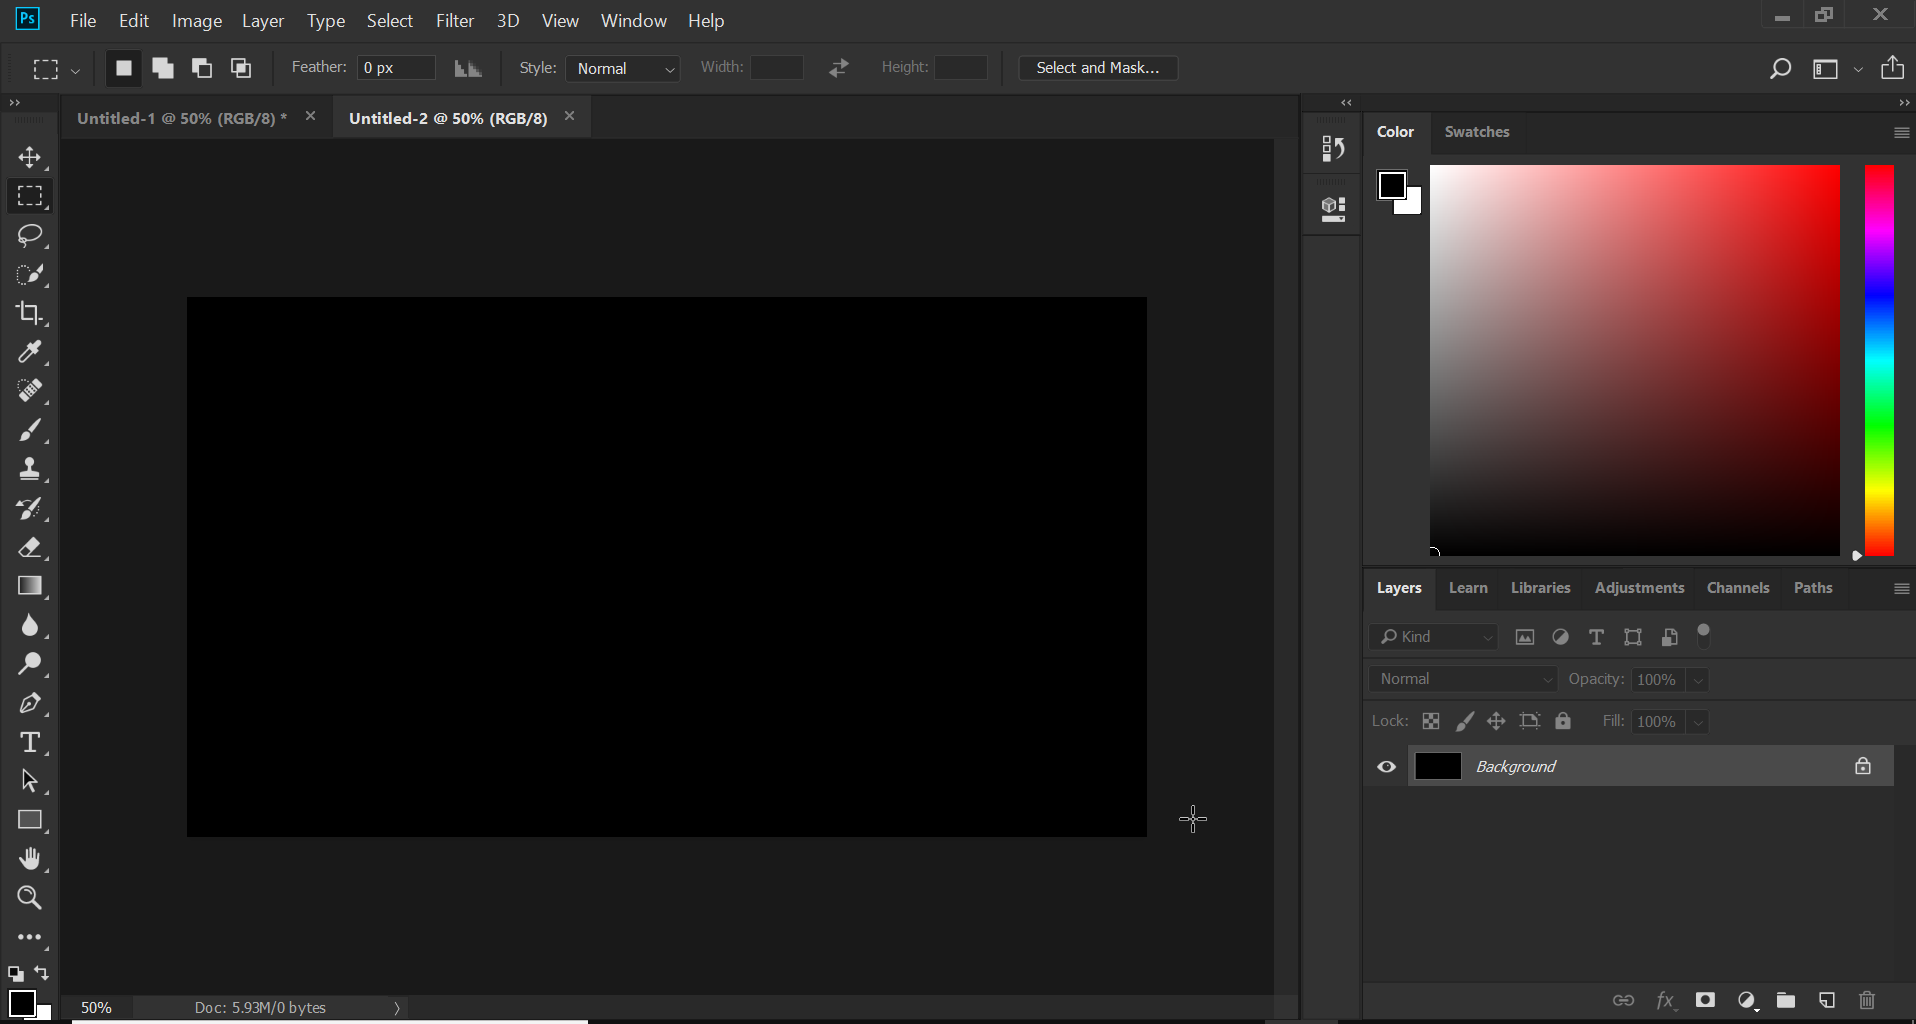
\includegraphics[width=.8\textwidth]{Figures/adobe-photoshop.png}
    \caption[Adobe Photostop]{Uživatelské rozhraní programu Adobe Photoshop}
    \label{fig:photoshop}
\end{figure}

\section{Google Web Designer}
Jedná se o propracovaný desktopový designer pro tvorbu HTML5 reklamních bannerů jak statických, tak animovaných.
S řadou předpřipravených šablon na míru již daných formátů reklamy poskytovaných Googlem je tento návrhář jedním z nejsilnějších
volně dostupných produktů pro tvorbu propagačních materiálů.

Umožňuje navázat na různé prvky banneru události a jednoduše tím udělat banner více interaktivní.
Dále zahrnuje možnost práci v 3D prostoru, nebo textovém HTML editoru.
Animace lze vytvořit pouhým přetažením objektů po plátně. Upravovat jde délka animace, trasa pohybu, časovací funkce apod.

Navíc program sám kontroluje řadu vlastností, které platforma Google Ads vyžaduje
(velikost souboru, validní HTML kód, správné URL odkazy atd.). Výslednou tvorbu je schopen přímo importovat do reklamní kampaně.
Vzhled programu lze vidět na obrázku \ref{fig:web-designer}.

\begin{figure}
    \centering
    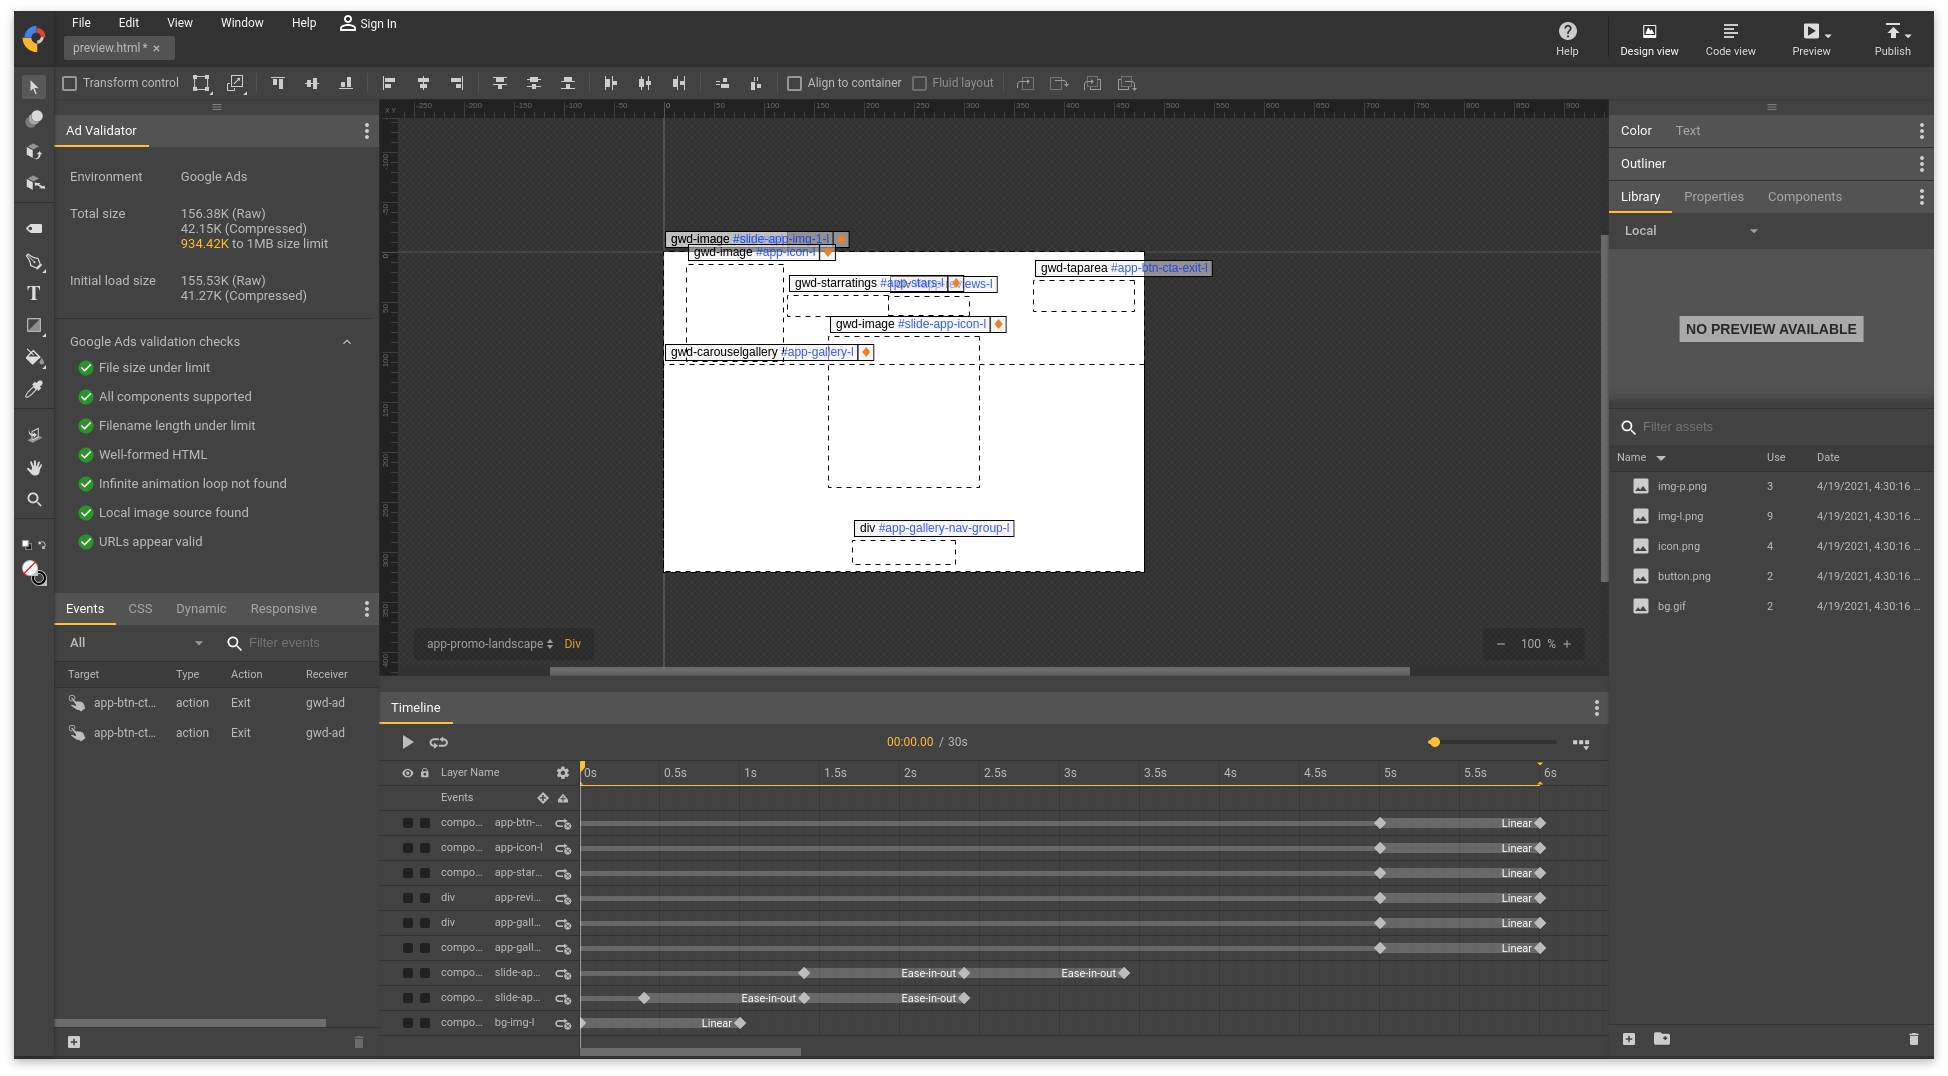
\includegraphics[width=.8\textwidth]{Figures/web-designer.png}
    \caption[Google Web Designer]{Uživatelské rozhraní programu Google Web Designer}
    \label{fig:web-designer}
\end{figure}

\section{Creatopy}
Tento online nástroj nabízí více svých pokročilých služeb pouze v placených verzích. Mezi jeho schopnosti však spadá vytváření HTML5 bannerů,
animací a tvorba více bannerů najednou. Poslední zmínění způsob tvorby je však limitován na pevně dané položky banneru jako logo, titulek,
tlačítko atd. Dále nabízí tvorbu Stories pro Facebook a Instagram. Na všechny možnosti poskytuje předpřipravené šablony,
které stačí upravit pro individuální potřebu.

Online editor nepoužívá pro práci element canvas, ale každý objekt je samostatný HTML element. Aplikováním kaskádových stylů je dosaženo požadovaného vzhledu.
To znamená, že možnosti úprav jsou dané možnostmi CSS, které v dnešní době sice zvládnou dostatečnou škálu efektů, jenže zavísí na podpoře prohlížečem.
Například, funkce \texttt{backdrop-filter} dokáže aplikovat různé filtry na pozadí HTML elementu, avšak zatím není v prohlížeči Firefox podporována.
Tím, že editor využívá práci přímo s HTML získává dobrou výkonnost, ale ztrácí, pokud si uživatel chce grafiku vytvořit sám.
Nástroj spoléhá spíše na využití mnoha předpřipravených tvarů, které se následně dají upravovat. Vytvořený banner umí následně zmenšit nebo
zvětšit na ostatní různé velikosti. Rozhraní aplikace je zobrazeno na obrázku \ref{fig:creatopy}.

\begin{figure}
    \centering
    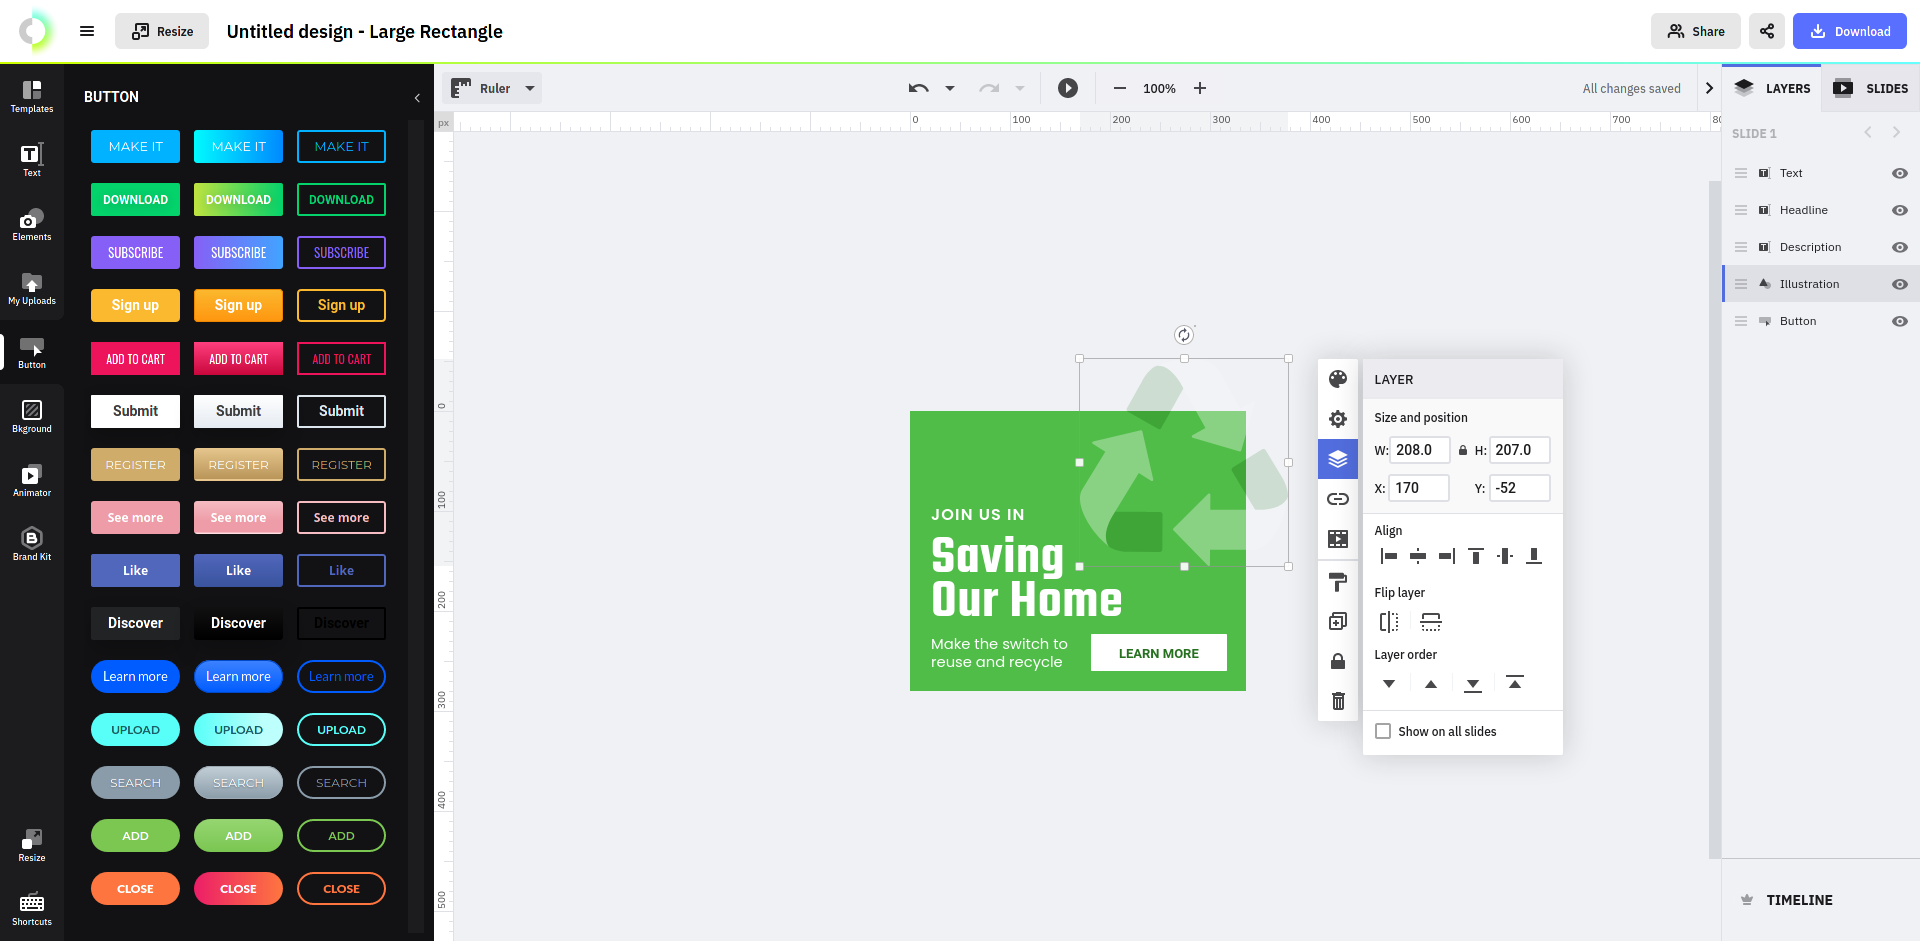
\includegraphics[width=.8\textwidth]{Figures/creatopy.png}
    \caption[Creatopy]{Uživatelské rozhraní aplikace Creatopy}
    \label{fig:creatopy}
\end{figure}


\section{Bannerflow}
Další prostředek tvorby bannerů prostřednictvím Internetu. Své služby nabízí v rámci předplatného.
Po zaplacení se uživatelům otevře jeden z nejpokročilejších nástrojů pro tvorbu online inzerce.
Samozřejmostí pro něj je návrh a zpracovaní grafiky. Bannery dokáže automaticky škálovat a obsah rozmístit v rámci libovolných velikostí.
Navíc oproti výše zmíněným službám umožňuje přímé napojení na hlavní poskytovatele reklamních sítí (nezmiňuje však konkrétně jaké) a
automatické nahrávání bannerů do reklamních kampaní. Dále také shromažďuje analytická data, které zpřístupňuje svým klientům přímo v rámci aplikace.

\section{Srovnání}
Ačkoli autor této práce hledal, nikde neuměl najít nástroj, který by umožnil jednoduše do stejné šablony bannerů nahrát zdroj dat textů a obrázků,
jehož výsledkem by byly bannery se stejným rozložením. Tato funkce může být vhodná například pro e-shopy,
které nabízí velké množství podobných produktů (pračky, sušičky, apod.). Pokud by tato možnost byla dostupná,
mohla by drasticky snížit celkový čas tvorby reklamy. 



\endinput